% !TeX root = ./main.tex

We now experimentally validate the performance of the different versions of our algorithm.
Our benchmarks were run on a compute cluster, where each explanation sequence generation was assigned a single core on a 10-core INTEL Xeon Gold 61482 (Skylake) processor, a timelimit of 120 minutes and a memory-limit of 4GB. 
Everything was implemented in Python on top of PySAT\footnote{\url{https://pysathq.github.io}} and is available at \url{https://github.com/ML-KULeuven/ocus-explain}. 
For MIP calls, we used Gurobi 9.0, for SAT calls MiniSat 2.2 and for MaxSAT calls RC2 as bundled with PySAT (version 0.1.6.dev11). In the MUS-based approach we used PySAT's deletion-based MUS extractor MUSX~\cite{marques2010minimal}.

All of our experiments were run on a direct translation to PySAT of the 10 puzzles of \citet{ecai/BogaertsGCG20}\footnote{In one of the puzzles, an error in the automatic translation of the natural language constraints was found and fixed.}. %Because of this error, it was missing in the experimental results of the previous work.} 
We used a cost of 60 for puzzle-agnostic constraints; 100 for puzzle-specific constraints; and cost 1 for facts.
When generating an explanation sequence for such puzzles, the unsatisfiable subset identifies which constraints and which previously derived facts should be combined to derive new information. 
%
Our experiments are designed to answer the following research questions: 
\begin{description}
 \item[Q1] What is the effect of requiring optimality of the generated MUSs on the \textbf{quality} of the generated explanations? 
 \item[Q2] Which \textbf{domain-specific \grow methods} perform best?
 \item[Q3] What is the effect of the use of \textbf{constrainedness} on the time required to compute an explanation sequence?
 \item[Q4] Does \textbf{re-use} of computed satisfiable subsets improve efficiency?
\end{description}

% \bart{too much detail... -> Requries explaingin what ``transtiivity'' etc mean in this setting) }\emilio{ok modified}

% \begin{figure}[ht]
%   \centering
%   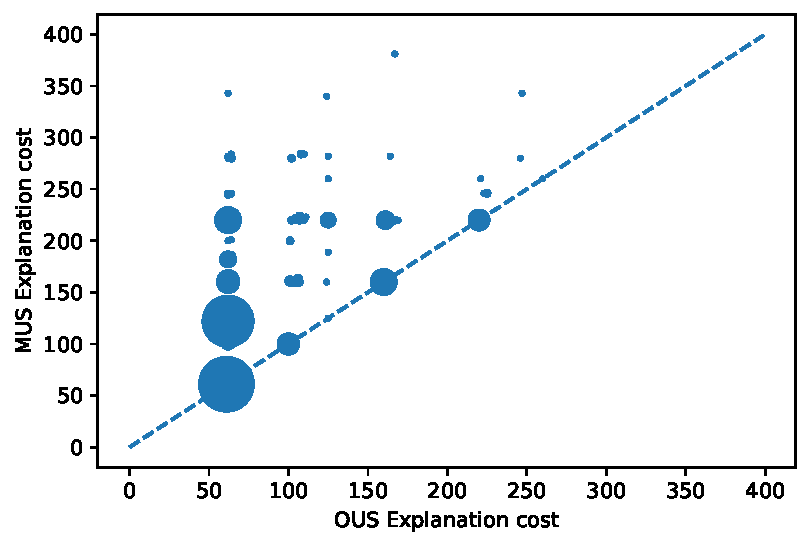
\includegraphics[width=\columnwidth]{figures/rq1.pdf}
%   \caption{Q1 - Optimal vs Greedy explanation generation quality}
%   \label{fig:rq1}
% \end{figure}

\begin{figure}[t]
  \centering
  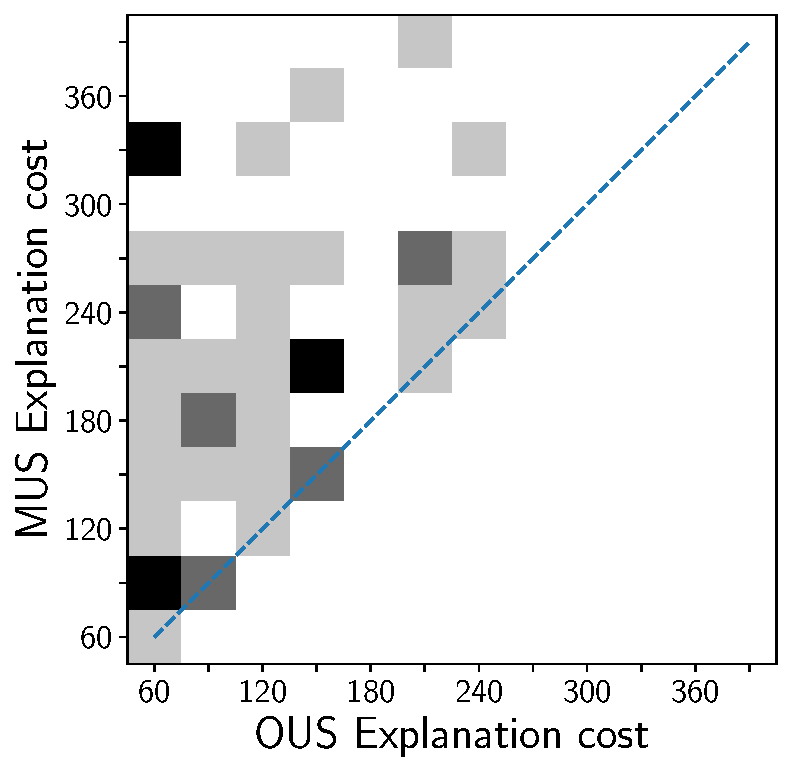
\includegraphics[width=0.6\columnwidth]{figures_post_paper/heatmap_costs_mus_cous.pdf}
  \caption{Q1 - Explanation quality comparison of optimal versus subset-minimal explanations in the generated puzzle explanation sequences.}
  \label{fig:rq1_heatmap}
\end{figure}


\paragraph{Explanation quality}\label{paragraph:explanationquality}
To evaluate the effect of optimality on the quality of the generated explanations, we reimplemented a MUS-based explanation generator based on \cref{alg:oneStep}. 
Before presenting the results, we want to stress that this is \emph{not} a fair comparison with the implementation of \citet{ecai/BogaertsGCG20}, since there --- in order to avoid the quality problems we will illustrate below ---  an extra inner loop was used that employs \emph{even more} calls to \call{MUS} for a selected set of subsets of \formulac of increasing size (this is their Algorithm~3). 
While this yields better explanations, it comes at the expense of computation time, thereby leading to several hours to generate the explanation of a single puzzle. 
%We will see in our later experiments is that we can both \emph{outperform}, in terms of computational cost, this simple \call{MUS} based implementation while also guaranteeing cost-optimality, as such achieving a Pareto improvement.

To answer \textbf{Q1}, we ran the \call{MUS}-based algorithm as described in \cref{alg:oneStep} and compared at every step the cost of the produced explanation with the cost of the optimal explanation. 
% 
% Similar to \citet{ecai/BogaertsGCG20}, a weight assigned to each type of constraint used. The weighted sum of the constraints present in the 
% (\textit{minimum} / \textit{optimal}) 
% minimal/optimal
% unsatisfiable subset become a proxy to how difficult the generated explanation really is.
% commaring the explanation quality of mus and ous
% To answer \textbf{Q1}, we start by generating a sequence of explanations using the \comus from an initial assignment $I_0$.. Then, using this sequence as a starting point, we look for a MUS-based explanation given the partial assignments $I_i$ at step i.
These costs are plotted on a heatmap in Figure \ref{fig:rq1_heatmap}, where the darkness represents the number of occurrences of the combination at hand. 
% Note that, the distribution of the dotts show the quality of the OUS explanation is either similar, when along the same-cost diagonal or better in the upper part of the graph. The dotts' sizes demonstrates 
We see that the difference in quality is striking in many cases, with the MUS-based solution often missing very cheap explanations (as seen by the two dark squares in the column around cost 60), thereby confirming the need for a cost-based \omus/\comus approach.
%\begin{table}[ht]
%		\centering
%	\begin{adjustbox}{max width=\columnwidth}
%\begin{tabular}{|c|c|c|c|c|}
%       \rule{0pt}{2ex} \textbf{MUS}& \textbf{OUS} &  \textbf{OUS+SS.Caching} &\textbf{OCUS} &  \textbf{OCUS+Incr.HS}\\
%        	\midrule
%	   \rule{0pt}{2ex}$90\pm23$ & $117\pm26$ & $113\pm15$   &  $119\pm22$ & $121\pm24$    \\
%	   	\bottomrule
%\end{tabular}
%	\end{adjustbox}
%\caption{Average number of explanation steps per config}
%\label{tab:config-number-explanation-steps}
%	\end{table}
% \tias{Please add avg (and maximum?) MUS size to show that 'smaller is not better' more explicitly}
%\paragraph{Notation} In the following, \emph{+SS. caching} corresponds to caching satisfiable subsets in order to re-use subsets between \omus calls, while \emph{+Incr.HS} corresponds to keeping the hitting set solver warm throughout the different calls to \onestepo.
%
%\begin{table}[!h]
%	\centering
%			\begin{adjustbox}{max width=\columnwidth}
%	\begin{tabular}{rrrrrr}
%%		 \cline{2-6}
%	& \multirow{2}{*}{\textbf{MUS}} & \multirow{2}{*}{\textbf{OUS}} &\textbf{OUS}  & \multirow{2}{*}{\textbf{OCUS}} &\textbf{OCUS}\\
%		\rule{0pt}{2ex}&  & & \textbf{+SS.Caching} &  & \textbf{+Incr.HS}  \\
%		\midrule
%\multicolumn{1}{r|}{\textbf{\textit{avg. $\#$ expl.}}} &  \textbf{90} &  117 &  113 &  119 &  121 \\
%%\multicolumn{1}{r|}{\rule{0pt}{3ex}\textbf{\textit{ $\overbar{\text{\# expl.}}$ }}} &  $90\pm23$ &  $117\pm26$ &  $113\pm15$ &  $119\pm22$ &  $121\pm24$ \\
%%\multicolumn{1}{|r|}{\rule{0pt}{2ex}\textbf{\textit{std. \# expl.}}} &  $23$ &   &  15 &  $22$ &  $24$ \\
%%		\hline
%\multicolumn{1}{r|}{\textbf{\rule{0pt}{2ex}\textit{max. expl. size}}} &  \textbf{14}&  13 & 13 &  13 &  13 \\
%\multicolumn{1}{r|}{\rule{0pt}{2ex}\textbf{\textit{avg. expl. size}}} &   \textbf{5.02} &   4.07 &   4.08 &  4.05 &   $4.07$ \\
%%\multicolumn{1}{|r|}{\rule{0pt}{2ex}\textbf{\textit{std-size}}} &   $2.08$ &   $1.47$ &   $1.47$ &   $1.42$ &   $1.41$ \\
%%\hline
%\multicolumn{1}{r|}{\rule{0pt}{2ex}\textbf{\textit{avg. $\#$ lits deriv.}}}&   \textbf{1.72} &   1.32 &   1.33 &   1.30 &   1.28 \\
%%\multicolumn{1}{|r|}{\rule{0pt}{2ex}\textbf{\textit{std lits deriv.}}} &   1.24 &   0.95 &   0.97 &   0.94 &   $0.91$ \\
%%\hline
%\bottomrule
%	\end{tabular}
%		\end{adjustbox}
%	\caption{\emilio{Statistics on the composition of the explanation sequences}}
%	\label{tab:config-number-explanation-steps-avg-max}
%\end{table}

%\begin{table}[!h]
%	\centering
%	\begin{adjustbox}{max width=\columnwidth}
%		\begin{tabular}{lrrrr}		
%			\toprule	
%			\textit{config} &\textbf{\textit{avg. \# expl.}} & \textbf{\textit{max. expl. size}} & \textbf{\textit{avg. expl. size}} &\textbf{\textit{avg. $\#$ lits deriv.}} \\
%			\midrule
%			\textbf{MUS} & 90& 14& 5.02 & 1.72\\
%			\midrule
%			\textbf{OUS} & 11 & 13& 4.07 & 1.32\\
%			\bottomrule
%			%		 \cline{2-6}
%			
%			%\multicolumn{1}{r|}{\rule{0pt}{3ex}\textbf{\textit{ $\overbar{\text{\# expl.}}$ }}} &  $90\pm23$ &  $117\pm26$ &  $113\pm15$ &  $119\pm22$ &  $121\pm24$ \\
%			%\multicolumn{1}{|r|}{\rule{0pt}{2ex}\textbf{\textit{std. \# expl.}}} &  $23$ &   &  15 &  $22$ &  $24$ \\
%			%		\hline
%%			\multicolumn{1}{r|}{\textbf{\rule{0pt}{2ex}\textit{max. expl. size}}} &  \textbf{14}&  13 & 13 &  13 &  13 \\
%%			\multicolumn{1}{r|}{\rule{0pt}{2ex}\textbf{\textit{avg. expl. size}}} &   \textbf{5.02} &   4.07 &   4.08 &  4.05 &   $4.07$ \\
%%			%\multicolumn{1}{|r|}{\rule{0pt}{2ex}\textbf{\textit{std-size}}} &   $2.08$ &   $1.47$ &   $1.47$ &   $1.42$ &   $1.41$ \\
%%			%\hline
%%			\multicolumn{1}{r|}{\rule{0pt}{2ex}\textbf{\textit{avg. $\#$ lits deriv.}}}&   \textbf{1.72} &   1.32 &   1.33 &   1.30 &   1.28 \\
%%			%\multicolumn{1}{|r|}{\rule{0pt}{2ex}\textbf{\textit{std lits deriv.}}} &   1.24 &   0.95 &   0.97 &   0.94 &   $0.91$ \\
%			%\hline
%			\bottomrule
%		\end{tabular}
%	\end{adjustbox}
%	\caption{\emilio{Statistics on the composition of the explanation sequences}}
%	\label{tab:config-number-explanation-steps-avg-max}
%\end{table}


%\begin{table}[ht]
%	\centering
%%		\begin{adjustbox}{max width=\columnwidth}
%\begin{tabular}{lrrrrr}
%	\cline{2-6}
%	&     \multicolumn{5}{c}{\textit{config}} \\
%	\cline{2-6}
%	\rule{0pt}{2ex} &     OCUS+I &       OCUS &      OUS+I &        OUS &        MUS \\
%	\midrule
%	max-size &  13 &  13 &  13 &  13 &  14 \\
%	avg-size &   4.07 &   4.05 &   4.08 &   4.07 &   5.02 \\
%	std-size &   1.41 &   1.41 &   1.47 &   1.47 &   2.08 \\
%	\bottomrule
%\end{tabular}
%%	\end{adjustbox}
%\caption{Average number of explanation steps per config}
%\label{tab:config-number-explanation-steps-avg-max}
%\end{table}

%\begin{table}[ht]
%	\centering
%			\begin{adjustbox}{max width=\columnwidth}
%	\begin{tabular}{cr|r|r|r|r|r|}
%		\cline{3-7}
%		&&     \multicolumn{5}{c|}{\textit{config}} \\
%		\cline{3-7}
%		\rule{0pt}{2ex}&  &     OCUS+I &       OCUS &      OUS+I &        OUS &        MUS \\
%		\hline
%	 \multicolumn{1}{|c|}{\multirow{3}{*}{\rotatebox[origin=c]{90}{\parbox[c]{1cm}{\centering MUS-size}}}}	& max &  13 &  13 &  13 &  13 &  14 \\
%	\multicolumn{1}{|c|}{}	& avg &   4.07 &   4.05 &   4.08 &   4.07 &   5.02 \\
%	\multicolumn{1}{|c|}{}	& std &   1.41 &   1.41 &   1.47 &   1.47 &   2.08 \\
%		\hline
%	\end{tabular}
%		\end{adjustbox}
%	\caption{Average number of explanation steps per config}
%	\label{tab:config-number-explanation-steps-avg-max}
%\end{table}

%<<<<<<< HEAD

%\paragraph{Explanation Sequence} \added{The effect of optimality is also noticeable on the quality of explanation sequence. The average number of explanations for MUS is 90, while \omus is at 117. 
%	The reason for this is that	the quality of the MUS-based explanations is worse compared to \omus. Worse explanations (that make more assumptions) often explain more literals at once and hence the total number of explanation steps is lower. 
%	In fact, on average a MUS-based explanation is composed of 5.02 constraints contrary to an \omus-based explanation with an average of 4.07 constraints.} \bart{Maar.... Dat zegt toch niets over de sequence...  Het enige dat hier staat is: doordat de individuele stappen minder goed zijn wordt de sequence korter. Dat zegt niets over of de sequence beter of slechter wordt. Welk punt wil je hier nog maken buiten ``de individuele stappen zijn slechter''? --> Ook: die averages: dat klopt ECHT niet met de heatmap. Een average OUS baserd ding kost onder de 150. Aangezien een constraint 60 of 100 kost, zou het average van OUS ongeveer 2.851215124 constraints moeten zijn. Geen 4. Waar komen die cijfers van? Zijn uw assen bij de figuur juist?}
	 %one of the two OUS implementations timed-out before completing the most difficult puzzle (hence explaining their lower number) and
	%To identify the effect on the quality of the generated explanation sequences, we report statistics on the generated sequences in Table \ref{tab:config-number-explanation-steps-avg-max} for MUS and OUS. 
	%The notation used in the table, is defined as follows: `avg. $\#$ expl.' is the average number of explanations in the explanation sequence; `max. expl. size' and `avg. expl. size' are respectively the maximum and average size of an explanation; avg. $\#$ lits derived is the average number of literals derived in an explanation. 
	%The average explanation size and literals derived in  \ref{tab:config-number-explanation-steps-avg-max} support the validity of this statement. 
%=======
%\emilio{Table \ref{tab:config-number-explanation-steps} provides additional information on the average number of explanation steps generated for each configuration. The average is not equal for all configurations, the reason for this is that one of the two OUS implementations timed-out before completing the most difficult puzzle (hence explaining their lower number) and the quality of the MUS-based explanations is worse. 
%	\tias{Too much talking. Keep only those that solved everything, actually just MUS and OUS (like in the figure) is sufficient to make the point of this experiment. Differences between OUS/OCUS raise questions, but are probably due to just different (random) ordering? if not shown, no need to explain here...} 
%	Worse explanations (that make more assumptions) often explain more literals at once and hence the total number of explanation steps is lower.
%>>>>>>> e4d5df1776ed855c31dae20748d5f394d39a4d9e

\paragraph{Domain-specific \grow} 
In our OCUS algorithm, we do not just aim to find any satisfiable subsets, but we prefer \emph{high quality} satisfiable subsets: subsets that impose strong constraints on the assignments the optimal hitting set solver can find. 
This induces a trade-off between \emph{efficiency} of the \grow strategy and \emph{quality} of the produced satisfiable subset.

\begin{figure}[ht]
  \centering
  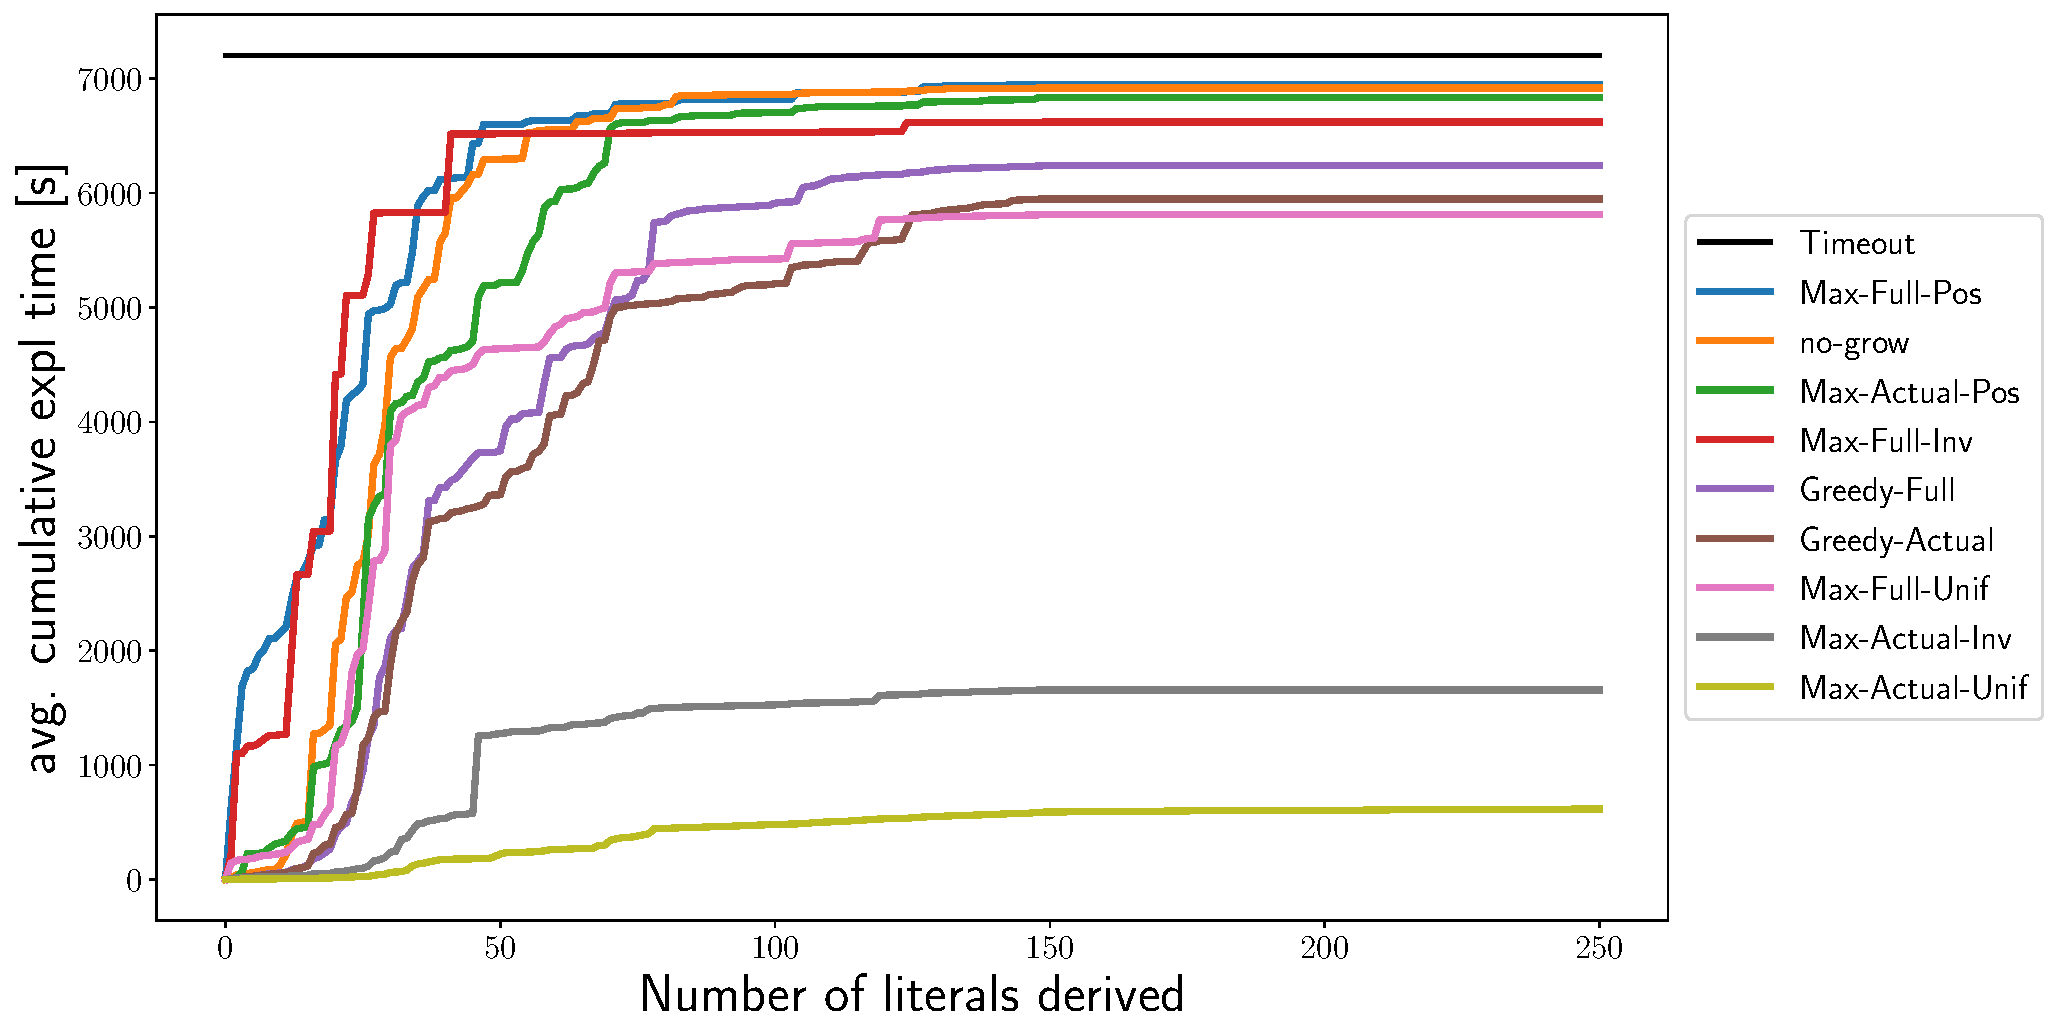
\includegraphics[width=\columnwidth]{figures_post_paper/new_cumul_grow_avg_time_lits_derived.pdf}
  \caption{Q2 - Explanation specific \grow strategies for \comus.}
  \label{fig:grow_strategies}
\end{figure}
% \tias{make 'Timeout' top entry of legend, sort legend according to ordering in graph}


%\deleted{Thus, to answer \textbf{Q2}, we depict in Figure \ref{fig:grow_strategies} the average of the cumulative explanation time of different \grow strategies to generate the explanation sequence of all puzzles combined
%	\tias{Be more specific: this is the average of the cumulative expl time for each puzzle? [not cumulative avg I think? you avg the cumulatives??}.}
Thus, to answer \textbf{Q2}, we compared variations of  \comus that only differ in which \grow strategy they use. 
Figure \ref{fig:grow_strategies} depicts the average (over all the puzzles) cumulative explanation time to derive a number of literals.
To compute the average, if a configuration time-outs on certain puzzle, we used the timeout time (7200s). 
The jump around literal 150 can be explained by the fact that there is only one puzzle with 250 literals, all others have at most 150. When a puzzle is finished, its final runtime is not taken into account in computing the average for the rest of the sequence \todo{IS THAT SO? In the current plot, if an instance time-outs at literl 50, its timeout is taken into account up to literal 150, but not beyond that? Sounds strange!}
% \bart{what are n-literals? Is this a typo? Or did you mean 
%\tias{This is specific for OCUS right? Or also for OUS? previous exp uses OUS, so say explicitly that for OCUS if so} 
The configurations are as follows:
\begin{itemize}
\item \emph{Max} refers to growing with a MaxSAT solver and \emph{Greedy} to growing using a heuristic method implemented by repeated sat calls. 
%\item 
\emph{no-grow} on the other refers to skipping \grow step.
\item  \emph{Full} refers to using the full unsatisfiable formula $\mathcal{F}$  while \emph{Actual} refers to using only the constraints that hold in the final interpretation (see Section~\ref{sec:ocusEx}). For instance, for the MaxSAT-based calls, using \emph{Actual} means that only the previously derived facts and the original constraints are taken into account when computing optimality. 
\item The \maxsat solver (\emph{Max}) is combined with different weighing schemes: uniform weights (\emph{unif}), original weights $w_i$, i.e., equal to the weights in the OCUS call (\emph{pos}) or the inverse of the original costs (\emph{inv}) defined as $max(w_i) + 1 - w_i$.% \bart{DEFINE INVERSE! What did you implement. } 
\end{itemize}
%\tias{switch explanation to follow names in figure: first explain Max vs greedy, then explain Actual vs Full, dan unif/inv/pos}.


%\tias{Use the names used in the figure, 'Max-Full variants'?}
As expected, the \maxsat-\grow on the actual interpretation \emph{Max-Actual} indeed performs best, though only \emph{Max-Actual-Unif} is able to finish all explanations. 
%When repeating this experiment for \omus the same pattern was observed. 
%\bart{AND also for incremental and non-incremental, right? Are you actually sure of that. We noticed this in the IJCAI paper but as far as I know, all your expiermental data from that time was messed up... } 
%The \emph{Greedy}-strategy provides some improvement on the cumulative runtime with respect to \emph{Max-Full}, but neither can generate explanations for all puzzle instances. \bart{Drop this last sentence?  Why focus on this?}}
%  \tias{broken sentence: what do you want to say? 'constrainedness' is not an option? or do you mean that similar results for OUS? be explicit, and if it does not contribute to the RQ then don't write it}.
% Notice in Figure~\ref{fig:grow_strategies} that only the \maxsat solver on actual variables and with uniform weights is able to complete the generation of a sequence for all puzzles. Furthermore, giving the \maxsat constraints on $\mathcal{F}$ drastically increases the execution time and, even within the best weighing scheme (\emph{unif}), it takes less than 10 steps\tias{how do you conclude this? non-obvious...} on average for every puzzle to time out.
%\tias{Should this not be: max-actual returns best results, through only max-actual-unif is able to finish all explanations. Greedy does better than max-full, but neither can solve all explanations)?}

%\deleted{
%We also observed (see \cref{tab:percentage_exec}) that in each of our configurations, the majority of the time is spent on computing hitting sets. As such, it makes sense to optimize the \grow procedure to provide results that are as good as possible and limit the choices of the hitting set solver as much as possible. 
%Slightly surprising, performing a \maxsat-\grow with the full interpretation takes \emph{less} time than on the actual interpretation. The gains of using the actual interpretation seems to come most from the fact that it generates better  sets to hit. 
%}
% \tias{TODO: explain table or cut}
%\begin{table}[t]
%  \centering
%  \resizebox{0.82\textwidth}{!}{\begin{minipage}{\textwidth}
%  		    \begin{tabular}{r|c|c|c|c|c}
%      %\hline
%      config &    $\#$HS &   $\%$HS &  $\%$SAT &  $\%$\grow & Time [s] \\
%      \hline
%      Greedy-SAT-Actual &   8679 &  89.0 &   0.0 &    9.0 &      66782 \\
%      Greedy-SAT-Full &   8787 &  88.0 &   0.0 &    10.0 &      66297 \\
%      Max-Actual-Unif &   6831 &  81.0 &   0.0 &   19.0 &       5449 \\
%      Max-Full-Unif &  17280 &  85.0 &   0.0 &   15.0 &      72000 \\
%      %\hline
%    \end{tabular}
%  \end{minipage}}
%  \caption{Number of hitting sets and total time (in seconds) spent in core parts of \comus algorithm across all puzzles.}
%  \label{tab:percentage_exec}
%\end{table}


% \tias{make 'Timeout' top entry of legend}

\paragraph{Constrainedness and incrementality}
To answer \textbf{Q3} and \textbf{Q4}, we compare the effect of constrainedness in the search for explanations (C), and incrementality for the \emph{Max-Actual-Unif} grow.
For \emph{OCUS}, incrementality (\emph{+Incr.~HS}) is achieved by keeping the hitting set solver warm throughout the explanation calls.  
To have a better view on how incrementality also affects \omus, we add incrementality in the following ways:
\begin{itemize}
	\item \emph{SS.~caching} keeps track of the satisfiable subsets internally and initialize \setstohit as presented in \cref{sec:ocusEx}.
	\item \emph{Lit.~Incr.~HS} keeps a hitting set solver warm for every literal to explain throughout the explanation calls. Once the literal is explained, the hitting set solver is discarded.
\end{itemize}
%To have a better view on how incrementality also affects \omus, we consider 3
% i.e., initialising the set of hitting sets ${\cal H}$ in an \omus call with the set of satisfiable subsets previously computed (+SS caching), and with reusing a single share hitting solvers across all OCUS calls (+Incr.HS). \bart{I cannot read this sentence. Waay too long. Also: why is a different method for incrementality used for OUS than for OCUS.}
%\bart{IMPORTAZTNT: ARE THESE RESULTS IN THE FIGURE EVEN CORRECT? I THOUGHT THAT IN THE LAST MEETING WE ROUGHLY CONCLUDED THAT OUS PLUS THE RIGHT INCREMENTAL STRATEGY WAS AS GOOD AS OCUS. NOW IT SUDDENLY IS NO LONGER THE CASE;}
% 
Figure \ref{fig:incrementality_constraindness} shows the results of the different variants, including the MUS-based variant discussed above. 
In this figure, the configurations are compared in a similar fashion to figure \ref{fig:grow_strategies}.
%\deleted{In this figure, the total number of explanation steps is not equal for all configurations, the reason for this is that the two OUS implementations timed-out before completing two of the puzzles (hence explaining their lower number) and the quality of the MUS-based explanations is worse, as observed in \textbf{Q1}. Worse explanations (that make more assumptions) often explain more literals at once and hence the total number of explanation steps is lower.}
%We choose to answers \textbf{Q3} and \textbf{Q4} using the cactus plot of Figure \ref{fig:incrementality_constraindness} with the same logarithmic scale for consistency. Furthermore, both incrementality and constraindness go hand in hand.
%All O(C)US variants use Max-Actual-Unif as \grow strategy following the results of the previous experiment.%, after we experimentally verified that this result of \textbf{Q2} also applied to the other OUS variants. %apply as well to all \mm{\call{O(C)US(+I)}} configurations illustrated on Figure \ref{fig:incrementality_constraindness}.
% \bart{This is confusing: the next paragraph contains 

\begin{figure}[t]
	\centering
	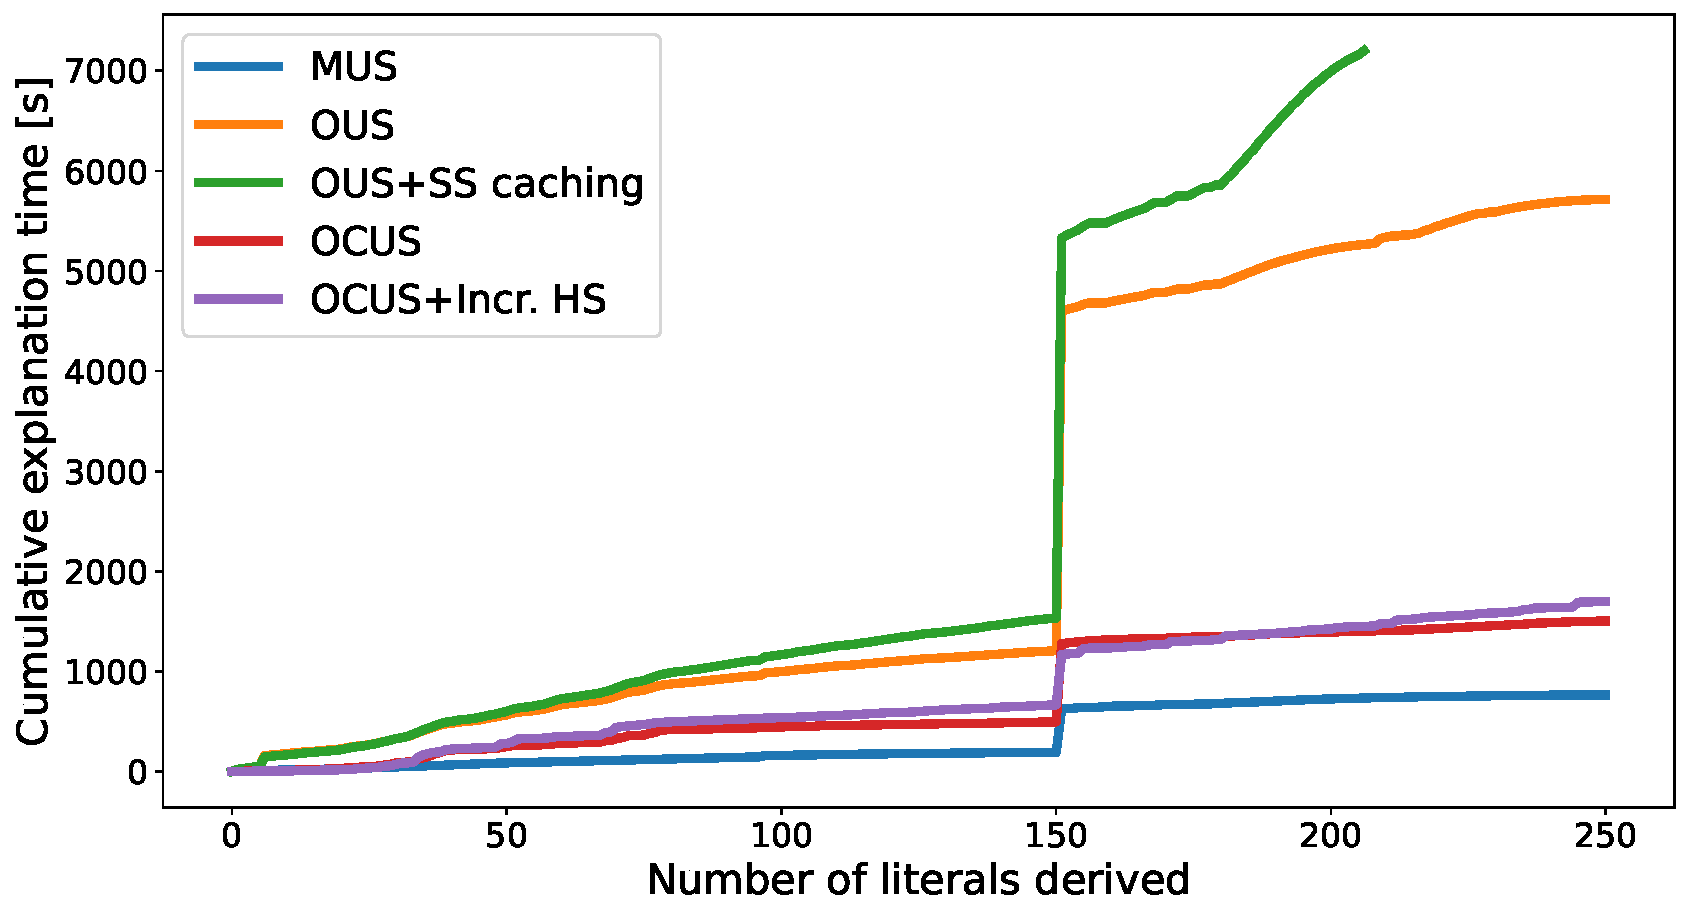
\includegraphics[width=\columnwidth]{figures_post_paper/cumul_incr_avg_time_lits_derived.pdf}
	\caption{Q3 - Cumulative runtime evolution enhancements on incrementality and constrainedness.}
	\label{fig:incrementality_constraindness}
\end{figure}

 \paragraph{Constrainedness}
When comparing all six configurations, we see that the \emph{O(C)US} implementations cannot keep up with the plain \emph{MUS}-based implementation, as is to be expected since a harder problem is tackled.
However, when using a single \textbf{constrained} (OCUS) call at every step we see a dramatic improvement in runtime. 
While slower than MUS, the runtime at most doubles, and, as investigated in \textbf{Q1} much better quality results are found. 
%. then multiple MUS calls,  ,  constrainedness, by switching to Algorithm \ref{alg:oneStepOCUS}, we effectively reduce the number of calls to the \omus solver.
%The constrainedness enhancement as shown in Figure \ref{fig:incrementality_constraindness} proves the importance of our approach.
%The explanation generation times for a whole sequence are on close to and sometimes even outperform  the MUS approach, while still solving the harder problem of unsatisfiable subset optimization. 

% Note that, for the same given puzzles, the number of explanations for MUS is lower COMUS, which supports the claim that the unsat subsets are of high cost as presented in \hyperref[paragraph:explanationquality]{explanation quality}.


% \paragraph{Incrementality}
% The naive, but optimal approach of pure 'OUS' requires notably more time than the non-optimal MUS-based algorithm. This observation demonstrates that the problem complexity increases when using an optimality criterion. We observe with 'OUS+I' that reusing information throughout the calls to the OUS solver burdens the \onestep algorithm with extra processing in order to keep track of all generated satisfiable subsets.

%%To our surprise, we noticed that \emilio{both in the constrained and non-constrained OUS setting, incrementality had no noticeable effect.
%%Even more so, naively restarting \textit{OUS} and \textit{OCUS} at every explanation step, without tracking the satisfiable subsets, provides improvements on the more difficult puzzles.
%%One potential explanation is when a branch-and-bound-based MIP solver such as Gurobi is kept warm, the solver will start in a search space close to the previous solution. However there is no immediate guarantee that the new best explanation is closely related to the previous one.}
\textbf{Incrementality} In the case of \comus, when using a single MIP solver and its built-in incrementality capabilities across all step, we see only minor runtime improvements at the end of the sequence where the more difficult steps are. Surprisingly, for \emph{OUS+Lit.~Incr.~HS} incrementality dramatically reduces the runtime with a runtime very close to \comus. For the first few literals, \emph{OUS+Lit.~Incr.~HS} is almost on par with \emph{MUS}.

%\bart


%leads to small runtime improvements in the intial steps \bart{In the initial steps??? That does not make sense. In the first step incremental or nonincremetnal should be the same}, which are not visible on the figure. When manually storing and initialising the set of satisfiable subsets, we can see that this induces an increasing overhead for later steps in the generation process that becomes substantial. In case of OCUS, when using a single MIP solver and its built-in incrementality capabilities across all steps, we can see small runtime improvements for some individual steps but on average it is slower in computing all explanations.

% 
%\deleted{When combining constrainedness with incrementality, on the other hand, we see that this incrementality yields important improvements. One potential explanation for this behaviour is the fact that, as discussed above, in the OCUS+I implementation, we only initialize a MIP and reuse it  across the different \onestep calls of algorithm \ref{alg:oneStepOCUS}.
%By keeping the MIP solver warm, we take advantage of its efficiency to handle the many satisfiable subsets which are represented under the form of constraints on the variables of the problem specification.
%Figure \ref{fig:incrementality_constraindness} demonstrates that contrary to \emph{OUS+I}, incrementality in \textbf{\comus+I} significantly decreases the overall computation time. }

%\ignore{
%\begin{table}[t]
%	\centering
%	\resizebox{0.82\textwidth}{!}{\begin{minipage}{\textwidth}
%			\begin{tabular}{r|c|c|c|c|c}
%				%\hline
%				config &    $\#$HS &   $\%$HS &  $\%$SAT &  $\%$\grow & Time [s] \\
%				\hline
%  Greedy-Sat-Actual &  80519 &  99.6 &   0.2 &    0.1 &    67753 \\
%Greedy-Sat-Full &  58791 &  99.7 &   0.1 &    0.1 &    69990 \\
%Max-Actual-Unif &  53728 &  59.1 &   0.8 &   37.3 &     5199 \\
%Max-Full-Unif &  32604 &  57.3 &   0.0 &   42.3 &    69900 \\
%				%\hline
%			\end{tabular}
%	\end{minipage}}
%	\caption{Number of hitting sets and total time (in seconds) spent in core parts of \emilio{not incremental} \comus algorithm across all puzzles.}
%	\label{tab:percentage_exec}
%\end{table}
%}
\begin{table}[!h]
	\centering
	\begin{adjustbox}{max width=\columnwidth}
\begin{tabular}{cccccccccc}
	Time [s] &\textbf{0-1} & \textbf{1-2} & \textbf{2-5} & \textbf{5-10} & \textbf{10-20} & \textbf{20-50} & \textbf{50-100} & \textbf{100-200} & \textbf{200-500}\\
	\midrule
	$\# expl$ &596 & 229 & 211 & 72 & 46 & 31 & 11 & 7 & 3\\
\end{tabular}
\end{adjustbox}
	\caption{Frequency of explanation-generation-time in the explanation sequence.}
	\label{tab:explanation-time}
\end{table}
%\begin{figure}[ht]
%	\centering
%	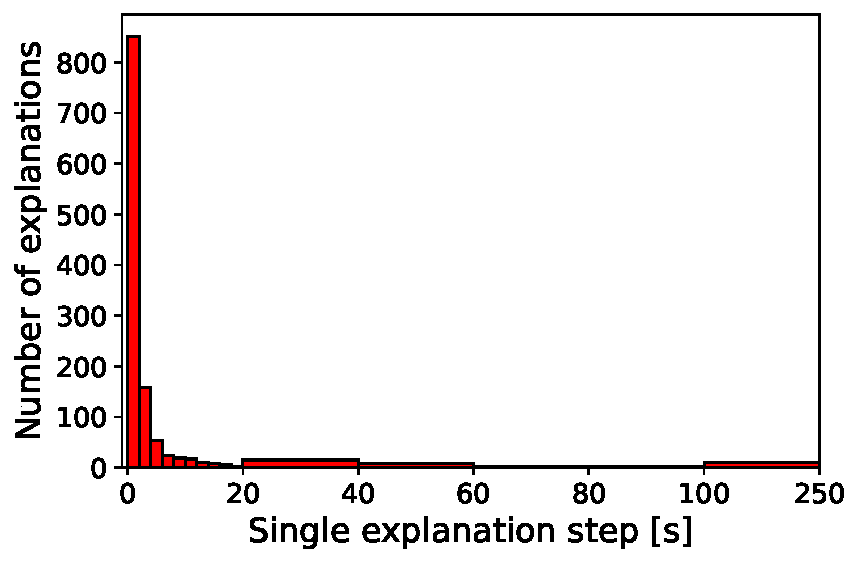
\includegraphics[width=\columnwidth]{figures_post_paper/explanation_times.pdf}
%	\caption{Distribution of the explanation generation time in the generated sequence.}
%	\label{fig:explanation_time}
%\end{figure}


%\bart{you have to say which conifguration this is done with}
As a final experiment, we investigate what the typical runtime is to explain one individual explain step for \emph{OCUS+Incr. HS} with \emph{Max-Actual-Unif} grow. 
This is shown in table \ref{tab:explanation-time}, where we can see that the major part of the explanations takes less than 2 to 5 seconds to be generated. On the other hand, a handful of explanations require 20 to 100+ seconds to be generated and dominated to total runtime for explaining a sequence. %Indeed, puzzles often involve many 'easy' derivation steps that involve few facts and constraints, and a few 'hard' derivation steps. Whether difficulty for a person solving a puzzle and an algorithm finding TRICKY... not writing it.

%\paragraph{Interactivity} \emilio{To analyze how the explanations compare in an interactive context, we represent a distribution of explanation generation times in figure \ref{fig:explanation_time}. We see that a major part of the explanations take less than 2 to 5 seconds to be generated. Even though, the difficult explanation steps can take more time ranging from 5 to 100+ seconds to be generated, it is only a small fraction of all generated explanations.}
%>>>>>>> e4d5df1776ed855c31dae20748d5f394d39a4d9e



%\todo{Add Discussion on the time to find optimal explanations}
% \resizebox{3cm}{!}{
%   \begin{minipage}
%     \begin{table}
%       \centering
%       \begin{tabular}{|r|c|c|c|c|c|}
%         \hline
%         config &    $\#$HS &   $\%$HS &  $\%$SAT &  $\%$Grow &  OCUS [s] \\
%         \hline
%         Greedy-Actual &   8679 &  89.0 &   9.0 &    0.0 &      66782 \\
%         Greedy-Full &   8787 &  88.0 &   10.0 &    0.0 &      66297 \\
%         Max-Actual-Unif &   6831 &  81.0 &   0.0 &   19.0 &       5449 \\
%         Max-Full-Unif &  17280 &  85.0 &   0.0 &   15.0 &      72000 \\
%         \hline
%       \end{tabular}
%       \caption{Time spent in core parts of \comus algorithm}
%     \end{table}
%   \end{minipage}
%   }
  

% \begin{figure}[ht]
%   \centering
%   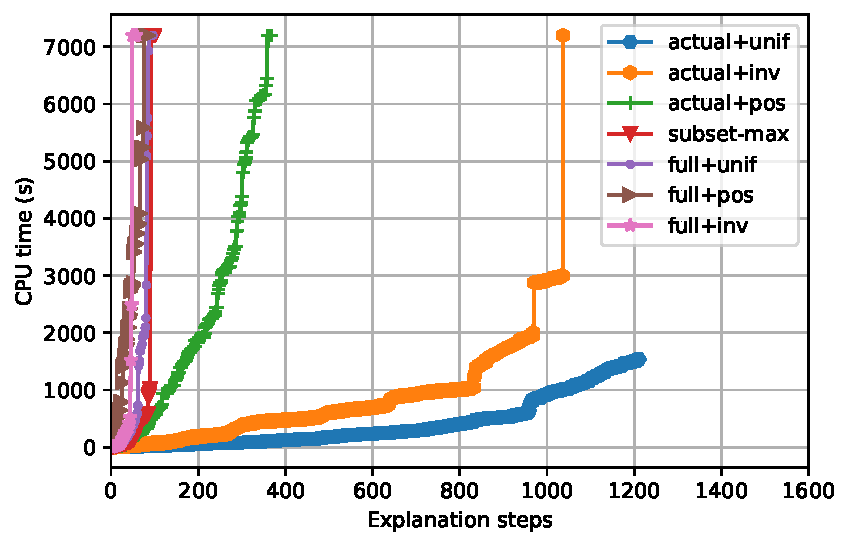
\includegraphics[width=\columnwidth]{figures/rq4.pdf}
%   \caption{Q4 - Grow strategies until timeout or full explanation sequence generation}
%   \label{fig:rq4}
% \end{figure}


% \begin{table*}[]
%     \centering
%     \caption{Execution time generic grow version}
%     \begin{tabular}{|r||c|c|c|c|c|}
%     \hline
%       p &             sat &          subset &      maxsat\_pos &     maxsat\_inv &    maxsat\_unif \\
%     \hline
%      6 &  15.25 - [18]  &  17.46 - [33]  &  48.41 - [9]  &  14.24 - [9]  &  14.71 - [16]  \\
%      8 &  38.95 - [6]  &  21.31 - [10]  &  1558.78 - [6]  &  14.26 - [6]  &  26.47 - [6]  \\
%      p &  14.09 - [9]  &  19.96 - [10]  &  646.94 - [9]  &  6.66 - [1]  &  9.84 - [4]  \\
%      2 &  18.6 - [9]  &  10.12 - [15]  &  171.94 - [9]  &  14.62 - [7]  &  16.54 - [7]  \\
%      7 &  10.24 - [7]  &  17.52 - [8]  &  1542.48 - [1]  &  13.03 - [1]  &  12.31 - [4]  \\
%      1 &  26.25 - [13]  &  20.52 - [13]  &  333.4 - [13]  &  13.28 - [12]  &  16.49 - [13]  \\
%      4 &  40.52 - [101]  &  22.86 - [108]  &  360.07 - [16]  &  14.18 - [11]  &  16.59 - [20]  \\
%      10 &  13.75 - [8]  &  26.72 - [8]  &  487.54 - [2]  &  17.88 - [4]  &  13.89 - [4]  \\
%      3 &  22.58 - [21]  &  19.57 - [10]  &  319.77 - [10]  &  13.49 - [9]  &  14.92 - [9]  \\
%     \hline
%     \end{tabular}
% \end{table*}





\ignore{\color{OliveGreen} old results to be removed
\begin{table}[ht]
  \centering
  \begin{tabular}{r||c|c|c|c|c}
    % \begin{tabular}{|r||c|c|c|c|c|c|}
      % \hline
      \textbf{p} & \textbf{MUS} & \textbf{OUS}  & \textbf{OUS+I} & \textbf{\comus} & \textbf{\comus+I} \\
      \hline
      1 &       569 &         4114 &     4727 &           803 &         \textbf{299} \\
      2 &       438 &         3834 &     3972 &           607 &         \textbf{238} \\
      3 &       477 &         4220 &     4938 &           932 &         \textbf{607} \\
      4 &       624 &         3508 &     4820 &           388 &          \textbf{97} \\
      5 &      3382 &         Timeout &     Timeout &          3556 &        \textbf{1537} \\
      6 &       568 &         3849 &     3854 &           498 &         \textbf{155} \\
      7 &       372 &         4411 &     4380 &           685 &         \textbf{414} \\
      8 &       474 &         4679 &     5552 &           669 &         \textbf{448} \\
      9 &       766 &         Timeout &     Timeout &          2383 &        \textbf{1135} \\
      p &       224 &         2601 &     2528 &           651 &         \textbf{537} \\
      % \hline
    \end{tabular}
    \caption{Computation time (s) compared between executions}
    \label{table:computationTime}
  \end{table}
}

\ignore{
We now experimentally validate the the performance of the different versions of our algorithms for explaining satisfiable constraint satisfaction problems.

We consider the following benchmarks: CNF instances from the SATLIB problems Benchmark \cite{hoos2000satlib} and a CNF encoding of the logic grid puzzle ``Origin'' of \cite{ecai/BogaertsGCG20}. All code was implemented in Python on top of %CPpy~\footnote{} and
PySAT.\footnote{\url{https://pysathq.github.io}} The MIP solver used is Gurobi 9.0 and when a (Max)SAT solver is used it is RC2 as bundled with PySAT. Experiments were run on a Intel(R) Xeon(R) CPU E3-1225 with 4 cores and 32 Gb memory, running linux 4.15.0.

Based on the theoretical findings of the previous sections, we aim to answer the following research questions:
\begin{compactdesc}
\item[RQ1] what is the effect of postponing optimal hitting set computation, of incremental OUS solving and of pre-seeding \satsets when solving multiple variants of the same problem?
\item[RQ2] how do the different variants of \omus perform when explaining an elaborate constraint satisfaction problem?
\ignore{
\item[RQ3] how do the sequences found when using (constrained) \omus search compare to those found using a heuristic MUS approach?
}
\end{compactdesc}


\paragraph{RQ1}
To answer the first research question, we use 10 CNF instances from the SATLIB Benchmark and randomly choose 10 literals that are entailed by the CNF. For each variant of the algorithm, we compute the OUS of the same 10 literals in the same order within a total time limit of 10 minutes. 
We compare the following enhancements options to the basic \omus algorithm: postponing optimization (+P), incrementality by reusing satisfiable subsets between \omus calls (+I), and pre-seeding $\satsets$ as described in Section~\ref{sec:incremental} (+W). Options can be combined, for example {\omus}+IPW characterises running the \omus algorithm postponing the optimization phase, with incrementality between the successive calls, and warm starting (pre-seeding) with satisfiable subsets of the original CNF formula.
%The executions are set to timeout after 10 minutes, a limit fixed based on the results of experiment 2.

% \rule{\textwidth}{10pt}

% \begin{table*}[t!]
%     \centering
%     \begin{tabular}{|c|c|c|c|c|c|c|c|c|}
%         \hline
%         % p    & nv& nc&           \omus &      {\omus}+Incr &      {\omus}+Post &  {\omus}+Incr+Warm &   {\omus}+Incr+Post & {\omus}+Incr+Post+Warm \\
%         p    & nv& nc&           \omus &      {\omus}+I &      {\omus}+P &  {\omus}+IW &   {\omus}+IP & {\omus}+IPW \\
%         \hline
%         aim-50-1\_6-yes1-4 & 50& 80&   0.88 s  &   0.38 s  &   0.37 s  &   0.81 s  &    0.65 s  &      \textbf{0.33} s  \\
%         par8-2 & 350 & 1157 &   122.42 s  &  94.07 s  &  96.84 s  &  120.55 s  &  126.15 s  &     \textbf{87.31} s  \\
%         zebra\_v155\_c1135 & 155& 1135&   130.38 s  &  87.97 s  &  84.75 s  &  104.7 s  &  124.48 s  &     \textbf{80.92 s}  \\
%         \hline
%         \end{tabular}
%         \caption{Execution time of the \omus variants for deriving 10 literals evaluated on CNF instances.}
%         \label{table:experiment1}
% \end{table*}

% \begin{table*}[t!]
%     \centering
%     \begin{tabular}{|c|c|c|c|c|c|c|c|c|}
%         \hline
%         % p    & nv& nc&           \omus &      {\omus}+Incr &      {\omus}+Post &  {\omus}+Incr+Warm &   {\omus}+Incr+Post & {\omus}+Incr+Post+Warm \\
%         p    & nv& nc&           \omus &      {\omus}+I &      {\omus}+P &  {\omus}+IW &   {\omus}+IP & {\omus}+IPW \\
%         \hline
%         % 1 & 50& 80&   0.88 s  &   0.38 s  &   0.37 s  &   0.81 s  &    0.65 s  &      \textbf{0.33} s  \\
%         % 2 & 350 & 1157 &   122.42 s  &  94.07 s  &  96.84 s  &  120.55 s  &  126.15 s  &     \textbf{87.31} s  \\
%         % 3 & 155& 1135&   130.38 s  &  87.97 s  &  84.75 s  &  104.7 s  &  124.48 s  &     \textbf{80.92 s}  \\
%         par8-5  & 350  & 1171&      --- &     --- &     --- &     --- &      --- &        --- \\
%         par16-1 & 317 & 1264           &      --- &  --- &  --- &     --- &      --- &     --- \\
%         par16-2& 349 & 1392         &      --- &     --- &     --- &     --- &      --- &        --- \\
%         par16-3 & 334 & 1332        &      --- &     --- &     --- &     --- &      --- &        --- \\
%         par16-4-c & 324 & 1292        &      --- &     --- &     --- &     --- &      --- &        --- \\
%         par16-4  & 1015 & 3324        &      --- &     --- &     --- &     --- &      --- &        --- \\
%         hanoi4  & 718 & 4934       &      1 &     1 &     1 &     1 &      1 &        1 \\
%         \hline
%         \end{tabular}
%         \caption{Number of decision variables explained by the variants of the \omus for timed-out CNF instances.}
%         \label{table:experiment1}
% \end{table*}

% \begin{table*}[t!]
%     \centering
%     \begin{tabular}{c|cccc|cccccc}
%         % \hline
%         p &  time [s] &  \#steps &   $\overline{cost}$ & max(cost) &    1 bij &  1trans &  1 clue & 1 clue+i & 1 mult-i & mult-c. \\
%         \hline
%         1 &  1287.27 &     115 &     25.87  &    25.87  &  31.83\% &  50.57\% &  1.09\% &    16.52 \% &     0\% &    0.0\% \\
%         % \hline
%         \end{tabular}
%         \caption{Puzzle Properties, execution statistics and explanation sequence composition for the origin puzzle.}
%         \label{table:experiment3}
% \end{table*}

% ------------------------------- EMILIO LOCK -----------------------------------------
The results can be seen in Table \ref{table:experiment1} and can be summarized as follows: p, nv and nc represent the instance name, the number of variables and the number of clauses respectively. 
Only for instances aim-50-1\_6-yes1-4, par8-2.cnf and zebra\_v155\_c1135.cnf, is the algorithm able to complete the search for OUSs on the 10 decision variables within the required time constraint of 10 minutes.
For these instances, the overall winner is \emph{{\omus}+IPW}. 
All variants time out on the larger instances (par8-5, par16-1, par16-2, par16-3, par16-4-c, par16-4, hanoi4) before finding the OUSs for all 10 decision variables. For instance par8-5, all variants are able to find 6 out of the 10 variables. On all instances that timed-out, \emph{{\omus}+IPW} remains the fastest. Similar results are observed for the remaining instances for all variants par16-* and hanoi4 with the \omus found for only 1 variable.


A further analysis of the overall execution times highlights that much time is spent in the \grow procedure, for which we start from the partial assignment found by the SAT check and use the RC2 MaxSAT solver to complete it. 
We reran the same experiments with a greedy \grow algorithm instead and observed that \omus is not even able to finish for zebra\_v155\_c1135 and all runtimes increase considerably.
Furthermore, we see that in this case postponing the MIP call effectively redistributes 50\% of the computational load to growing \satsets and the remaining 50 \% are evenly distributed between (i) the SAT solver, (ii) the MIP solver, and (iii) the the greedy and incremental hitting set heuristics. Hence, while the portion of time spent growing satisfiable subsets is reduced, much more iterations are needed to find the optimal OUSs. %runtime of grow is decreased, the number of 
% A further analysis of the overall execution times highlights that the main bottleneck of the algorithm is the time spent WE NEED TEXT HERE AFTER TEH RUNS ARE READY\todo{emilio}

From this experiment we conclude that in the short time limit provided, the best configuration for computing multiple related OUS's is \emph{{\omus}+IPW}, taking advantage of the repeated calls to the OUS algorithm, thus reusing the computed \satsets.
% ------------------------------- EMILIO LOCK -----------------------------------------

% \begin{table*}[h!]
%     \begin{tabular}{|c|c|c|c|c|c|c|c|c|}
%         \hline
%         % p    & nv& nc&           \omus &      {\omus}+Incr &      {\omus}+Post &  {\omus}+Incr+Warm &   {\omus}+Incr+Post & {\omus}+Incr+Post+Warm \\
%         p    & nv& nc&           \omus &      {\omus}+I &      {\omus}+P &  {\omus}+IW &   {\omus}+IP & {\omus}+IPW \\
%         \hline
%         1 & 50& 80&   0.88 s  &   0.38 s  &   0.27 s  &   0.81 s  &    0.65 s  &      0.33 s  \\
%         2 & 350 & 1157 &   22.42 s  &  14.07 s  &  76.84 s  &  20.55 s  &  126.15 s  &     87.31 s  \\
%         3 & 155& 1135&   130.38 s  &  87.97 s  &  64.75 s  &  104.7 s  &  124.48 s  &     80.92 s  \\
%         4..10 & x $\cdot$ $10^2$ & x $\cdot$ $10^3$           &      --- &     --- &   --- &  --- &   --- &     --- \\
%         % 5 & 317 & 1264           &      --- &  --- &  --- &     --- &      --- &     --- \\
%         % 6 & 324 & 1292        &      --- &     --- &     --- &     --- &      --- &        --- \\
%         % 7 & 334 & 1332        &      --- &     --- &     --- &     --- &      --- &        --- \\
%         % 8& 349 & 1392         &      --- &     --- &     --- &     --- &      --- &        --- \\
%         % 9  & 1015 & 3324        &      --- &     --- &     --- &     --- &      --- &        --- \\
%         % 10  & 718 & 4934       &      --- &     --- &     --- &     --- &      --- &        --- \\
%         \hline
%         \end{tabular}
%         \caption{Comparison of \omus variants evaluated on CNF instances.}
%         \label{table:experiment1}
% \end{table*}

% \begin{table*}
%     \begin{tabular}{|c|c|c|c|c|c|c|}
%         \hline
%         p                  &           \omus &      {\omus}+Incr &      {\omus}+Post &  {\omus}+Incr+Warm &   {\omus}+Incr+Post & {\omus}+Incr+Post+Warm \\
%         \hline
%         1 &    0.88 s | 10 &   0.38 s | 10 &   0.27 s | 10 &   0.81 s | 10 &    0.65 s | 10 &      0.33 s | 10 \\
%         2            &   22.42 s | 10 &  14.07 s | 10 &  76.84 s | 10 &  20.55 s | 10 &  126.15 s | 10 &     87.31 s | 10 \\
%         3  &  130.38 s | 10 &  87.97 s | 10 &  64.75 s | 10 &  154.7 s | 10 &  124.48 s | 10 &     80.92 s | 10 \\
%         4            &      600 s | 1 &  600 s | 2 &  600 s | 1 &     600 s | 1 &      600 s | 1 &     600 s | 1 \\
%         5         &      600 s | 1 &     600 s | 1 &     600 s | 1 &     600 s | 1 &      600 s | 1 &        600 s | 1 \\
%         6         &      600 s | 1 &     600 s | 1 &     600 s | 1 &     600 s | 1 &      600 s | 1 &        600 s | 1 \\
%         7         &      600 s | 1 &     600 s | 1 &     600 s | 1 &     600 s | 1 &      600 s | 1 &        600 s | 1 \\
%         8          &      600 s | 6 &     600 s | 6 &     600 s | 2 &     600 s | 6 &      600 s | 2 &        600 s | 2 \\
%         9         &      600 s | 1 &     600 s | 1 &     600 s | 1 &     600 s | 1 &      600 s | 1 &        600 s | 1 \\
%         10            &      600 s | 6 &     600 s | 6 &   600 s | 6 &  600 s | 6 &   600 s | 6 &     600 s | 6 \\
%         \hline
%         \end{tabular}
%         \caption{Comparison of \omus variants evaluated on CNF instances.}
%         \label{table:experiment1}
% \end{table*}


\paragraph{RQ2}
The second research question is: how do the different variants perform when explaining an elaborate constraint satisfaction problem? For this, we tested the complete generation of an explanation sequence. 
In this comparison, we expect that constrained versions of our algorithm perform best as they will allow performing an entire step of the explanations in a single call.
For this reason, we only include different variations on the constrained configuration and the single best variant of non-constrained algorithms found in the previous experiment. 

% \begin{figure}[t]
%     \centering
%     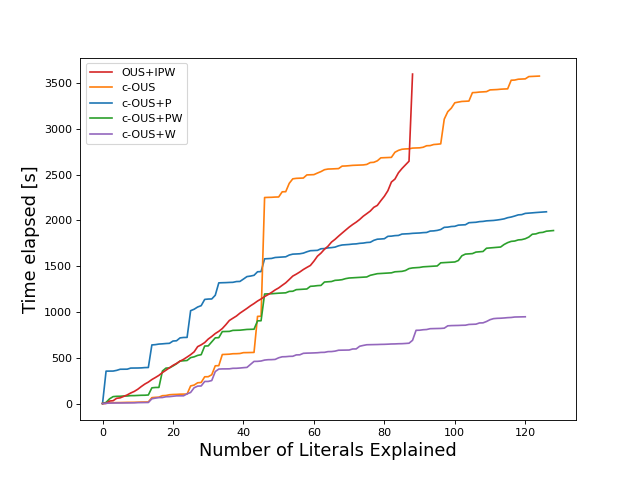
\includegraphics[width=\columnwidth]{figures/omusConstrCumulative.png}
%     \caption{Experiment 2}
%     \label{fig:exp2}
% \end{figure}

We generate the explanation sequence as far as possible within a time limit of one hour. 
The results for the  ``origin'' puzzle is shown in Figure~\ref{fig:exp2}.
It shows the number of literals explained on the X-axis, and the cumulative time taken on the Y-axis. 
Only three configurations find the full explanation sequence (note that there can be multiple optimal sequences with a different length, which explains the difference in length between the configurations).
We  see that the best non-constrained implementation is unable to explain all of the literals within the time limit; especially around step 95 there is a big jump in runtime. The vanilla constrained-OUS approach is not able to finish in time either, with big jumps in time on specific (large and costly) explanation steps.

When combining constrained-OUS with either pre-seeding, post-poned optimisation or both, then our approach is able to fully explain the solution. Best results are obtained with constrained-OUS with just pre-seeding at the beginning. The post-poned optimisation in this case may spent a lot of time generating MCSs that are not or little relevant to the constrained OUSs we are seeking. 

\paragraph{Concluding notes}
While a direct comparison of the runtime needed to find an explanation sequence of our tool versus the one of \citet{ecai/BogaertsGCG20} %built on the IDP system \cite{WarrenBook/DeCatBBD14} 
would shed more light on the performance impact, we can not do a fair comparison as the solvers and hardware used are different.

However, the authors reported that explaining a single puzzle easily takes one to two hours due to the many MUS calls. In contrast, Figure~\ref{fig:exp2} shows that three of our constrained-OMUS approaches fully explain a puzzle one of their larger puzzles in 20 to 30 minutes.
Furthermore, our algorithms guarantee that each explanation step is \emph{optimal} with respect to $f$. As such we know that the generated sequences are at least as good for the cost function provided.

% do not include such an extensive experiment here since it would not be a fair comparison of the underlying algorithms. Indeed, different solving technology is used for finding MUSs, and satisfying assignments. 
%We can, however, give an indication of the speed by mentioning that in some preliminary experiments (e.g., on the origin puzzle), using constrained \omus calls, we can find the entire sequence in roughly 20 minutes, whereas the IDP-based tool takes over two hours.


% Finally, for \textbf{RQ3} \emilio{Bart: concluding phrases on expl. generation}
%  we compare the sequence found by our proposed method with the sequence reported on in~\cite{ecai/BogaertsGCG20} for the origin puzzle (puzzle 1). 
% The explanation sequence for the puzzle is generated using \omus Constr with pre-seeding and according to the same cost function as Bogaerts et al.~\cite{ecai/BogaertsGCG20}. We report statistics relating to the explanation generation in table~\ref{table:experiment3}.
% Evidently, one of the most important observations is the speed-up provided by \omus Constr. 
% As a matter of fact, the sequence is generated in a bit more than 21 minutes compared to a few (2-3) hours in~\cite{ecai/BogaertsGCG20}, meaning that \omus Constr is 8-10x faster, while also finding the optimal explanations in each step.
% Table \ref{table:experiment3} also reports that the explanation sequence has become easier to understand: the average cost is slightly lower and so is $max(cost)$, the cost of the most difficult explanation in the puzzle. 


% \begin{table*}
%     \begin{tabular}{ccc|ccc|cccccc}
%         % \hline
%         types &  $|dom|$ &  $|grid|$ &  time [s] &  \#steps &    cost &    1 bij &  1trans &  1 clue & 1 clue+i & 1 mult-i & mult-c. \\
%         \hline
%         4 &      5 &     150 &  1287.27 &     115 &        25.87 &  27.83\% &  49.57\% &  6.09\% &    11.3\% &     5.22\% &    0.0\% \\
%         % \hline
%         \end{tabular}
%         \caption{Puzzle Properties, execution statistics and explanation sequence composition for the origin puzzle.}
%         \label{table:experiment3}
% \end{table*}

%
%\begin{figure*}[ht]
%    \centering
%    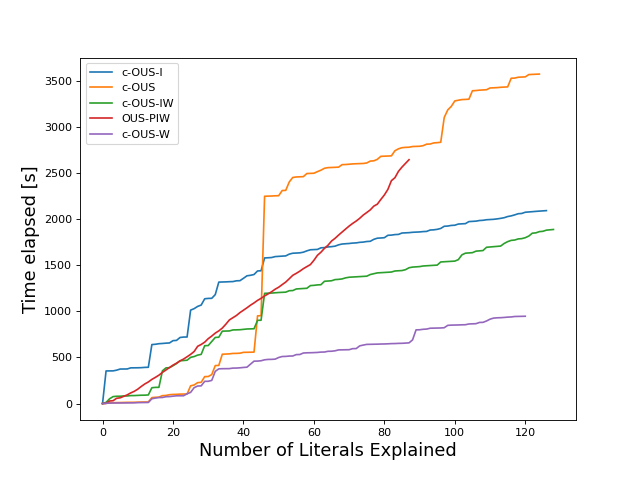
\includegraphics[width=\columnwidth]{figures/omusNonConstrCumulative.png}
%    \caption{}
%    \label{}
%\end{figure*}

% \begin{figure}[ht]
%     \centering
%     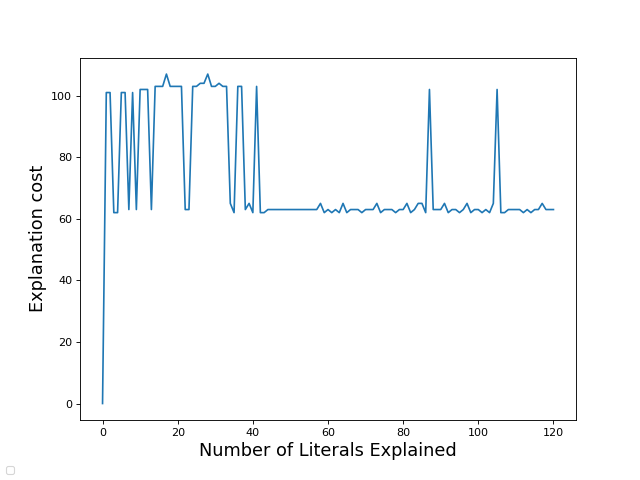
\includegraphics[width=\columnwidth]{figures/explanation_cost.png}
%     \caption{}
%     \label{}
% \end{figure}

}
